% !Mode:: "TeX:UTF-8"
% !TEX program = xelatex

\documentclass{report}

\usepackage{amsmath}
\usepackage{booktabs}
\usepackage{graphicx}
\usepackage{multirow}
\usepackage{array}
\usepackage{tikz}
\usepackage{pgfplots}
\usepackage{float}
\usetikzlibrary{arrows.meta,positioning,fit,calc}
\pgfplotsset{compat=1.17}

\title{基于Transformer的城市道路场景语义分割复现与边界增强改进}
\stunum{第*组}
\stuname{张三、李四、王五}
\stuclass{计算机科学与技术20**级*班}
\supervisor{**** \hspace{1.0em} 老师}
\dateinput{\today}

\begin{document}

\maketitle

\pagestyle{plain}
\pagenumbering{Roman}
\tableofcontents
\newpage
\pagestyle{plain}

\setcounter{page}{1}
\pagenumbering{arabic}

\section{团队成员分工}

本课程设计围绕城市道路场景语义分割问题展开，主要完成近五年代表性论文精读、官方代码结构分析、核心算法复现思路设计、模拟实验结果构造与对比分析、改进方法设计以及报告撰写等工作。团队成员分工如下：

\begin{itemize}
    \item 张三：负责语义分割研究背景调研、SegFormer论文精读、MiT编码器与MLP解码器原理分析。
    \item 李四：负责Mask2Former、PIDNet、Segment Anything论文阅读，整理近年分割方法的发展脉络与官方代码结构。
    \item 王五：负责实验主线设计、模拟复现实验数据整理、边界增强改进方案设计、图表绘制与报告整合。
\end{itemize}

若以个人形式完成，可将以上分工调整为“本人独立完成文献调研、算法分析、实验模拟、图表绘制和报告撰写”。

\section{任务背景}

语义分割是计算机视觉领域中的一类典型密集预测任务，其目标是为图像中的每一个像素分配一个语义类别标签。与图像分类只判断整幅图像所属类别不同，语义分割需要同时理解图像中的物体类别、空间位置和边界形状，因此在自动驾驶、智能交通、移动机器人、遥感影像分析、医学图像处理等场景中具有重要价值。在城市道路场景中，感知系统需要识别道路、车道、人行道、车辆、行人、建筑、天空和交通标志等不同区域。若分割边界不准确，可能造成道路边缘误判、小目标漏检或动态障碍物识别错误，从而影响后续路径规划和安全决策。

早期语义分割方法主要依赖手工特征和传统分类器，例如超像素、条件随机场和随机森林等。深度学习兴起后，Fully Convolutional Network将分类网络中的全连接层替换为卷积层，使网络能够输出空间分辨率较高的像素级预测图，成为深度语义分割的重要起点。随后，UNet通过编码器和解码器之间的跳跃连接增强了细节恢复能力，DeepLab系列利用空洞卷积和空间金字塔池化扩大感受野，PSPNet通过金字塔池化聚合全局上下文。这些CNN方法在相当长时间内占据主流，但卷积运算具有局部感受野，虽然可以通过堆叠层数扩大上下文范围，却仍然存在全局依赖建模效率不足的问题。

近五年来，Transformer在视觉任务中快速发展。Vision Transformer将图像划分为patch并利用自注意力建模长距离依赖，证明了纯Transformer结构在图像识别中的可行性。对于语义分割这类密集预测任务，研究者进一步提出了层次化Transformer、多尺度特征融合、mask classification和视觉基础模型等方向。SegFormer提出了Mix Transformer编码器和轻量MLP解码器，在精度和效率之间取得良好平衡\cite{segformer}；Mask2Former将语义分割、实例分割和全景分割统一到mask分类框架中\cite{mask2former}；PIDNet从实时分割需求出发，引入类似PID控制的三分支设计，强调边界分支对道路场景的重要性\cite{pidnet}；Segment Anything则通过大规模数据和提示式分割展示了视觉基础模型的发展趋势\cite{sam}。

本课程设计选择“基于Transformer的城市道路场景语义分割复现与边界增强改进”作为主题，原因有三点。第一，语义分割是计算机视觉中的基础问题，算法原理清晰且实验评价体系成熟。第二，SegFormer、Mask2Former、PIDNet和SAM均为近五年具有代表性的成果，能够覆盖高效Transformer、统一分割框架、实时分割和基础模型等不同技术路线。第三，道路场景对边界质量要求较高，适合在现有模型基础上提出轻量改进，即在SegFormer解码端加入边界增强分支，通过边界监督改善车辆轮廓、道路边缘和行人等区域的分割质量。

\section{任务描述}

本文研究的具体任务是城市道路场景语义分割。给定一幅道路场景RGB图像，模型需要输出与输入图像空间尺寸对应的语义标签图，每个像素被分配到道路、建筑、天空、车辆、行人、人行道、树木、交通标志等类别之一。该任务本质上是像素级多分类问题，其难点主要体现在以下几个方面。

第一，城市道路图像具有复杂的尺度变化。同一图像中既可能包含大面积道路和天空，也可能存在远处车辆、行人和交通标志等小目标。第二，类别之间边界细节复杂，例如道路和人行道、车辆和背景、行人和建筑之间经常存在细窄边缘区域。第三，不同天气、光照、遮挡和视角会造成明显外观变化，使模型需要具备较强的上下文理解能力和泛化能力。第四，在实际智能交通场景中，算法不仅需要准确，还需要较高推理速度，这要求模型在精度和效率之间取得平衡。

本文的工作目标包括：

\begin{enumerate}
    \item 查阅并精读近五年语义分割领域的代表性论文，重点分析SegFormer、Mask2Former、PIDNet和Segment Anything的理论原理、网络结构和算法特点。
    \item 主动研究论文附带的GitHub官方代码，整理其核心模块、训练入口、推理流程和与论文原理之间的对应关系。
    \item 以SegFormer-B0作为主要复现对象，分析其Mix Transformer编码器、空间缩减注意力和MLP解码器的实现方式。
    \item 基于官方论文结果和代码结构，采用模拟分析的方式构造实验主线，不在本机环境进行完整训练，重点比较不同方法的精度、速度和边界质量趋势。
    \item 借鉴PIDNet的边界辅助思想，提出SegFormer-B0 + Boundary Head改进结构，并通过模拟消融实验分析边界监督对分割结果的影响。
    \item 明确区分已有工作和本文设计工作：SegFormer、Mask2Former、PIDNet和SAM的主体算法属于已有论文成果；本文的工作是在SegFormer复现框架上设计轻量边界增强分支，并围绕该结构完成模拟实验分析。
\end{enumerate}

\section{技术方案}

\subsection{方案总体架构}

本文总体技术路线如图\ref{fig:pipeline}所示。首先进行文献调研和官方代码分析，确定SegFormer-B0为主要复现模型；其次构建实验方案，包括数据集设定、评价指标、基线模型、主模型和改进模型；然后围绕边界增强思想设计轻量分支和联合损失函数；最后通过模拟对比实验、消融实验和定性分析，讨论不同方法的优势与不足。

\begin{figure}[H]
\centering
\begin{tikzpicture}[
    node distance=1.1cm and 1.2cm,
    block/.style={draw, rounded corners=2pt, align=center, minimum height=0.85cm, minimum width=2.6cm, fill=gray!10},
    arrow/.style={-Latex, thick}
]
\node[block] (paper) {论文精读\\SegFormer等};
\node[block, right=of paper] (code) {官方代码分析\\模块映射};
\node[block, right=of code] (model) {SegFormer-B0\\模拟复现};
\node[block, below=of model] (edge) {边界增强分支\\本文改进};
\node[block, left=of edge] (exp) {对比实验\\消融实验};
\node[block, left=of exp] (report) {结论分析\\报告撰写};
\draw[arrow] (paper) -- (code);
\draw[arrow] (code) -- (model);
\draw[arrow] (model) -- (edge);
\draw[arrow] (edge) -- (exp);
\draw[arrow] (exp) -- (report);
\end{tikzpicture}
\caption{本文课程设计总体流程}
\label{fig:pipeline}
\end{figure}

由于本课程设计不在本机环境运行训练程序，实验部分采用“官方代码结构分析 + 公开论文结果趋势 + 可解释模拟实验”的方式完成。该方式的重点不是宣称获得新的真实训练指标，而是通过结构拆解、指标对照和消融设置，说明不同算法设计对语义分割精度、速度和边界质量的影响。

\subsection{代表性论文与方法分析}

\subsubsection{SegFormer}

SegFormer是本文的核心复现对象。该方法针对视觉Transformer在语义分割中的两个问题进行了改进：一是普通ViT缺少适合密集预测的多尺度特征，二是固定位置编码会限制模型在不同输入分辨率上的泛化。SegFormer提出Mix Transformer编码器，通过四个stage逐级降低特征图分辨率并提升通道数，得到类似CNN主干的层次化多尺度特征。同时，SegFormer不使用显式位置编码，而是在MLP模块中加入depth-wise convolution，使模型能够在保留灵活输入尺寸的同时获得局部位置信息。

SegFormer编码器中的注意力模块采用空间缩减策略。对输入特征$X$计算query时保持原空间分辨率，而对key和value进行降采样，从而降低自注意力计算复杂度。若原始token数量为$N$，缩减比例为$R$，则key和value的长度约变为$N/R^2$，注意力复杂度由$O(N^2)$降低为$O(N^2/R^2)$。这种设计对高分辨率语义分割任务非常重要，因为密集预测需要保留较大的特征图。

SegFormer解码器则非常轻量。它将四个stage输出的特征分别通过MLP投影到统一维度，再上采样到相同空间尺寸并拼接融合，最后用$1 \times 1$卷积输出类别logits。与DeepLabV3+等复杂解码器相比，SegFormer的解码器结构简单，参数量小，能够减少计算开销。本文选择SegFormer-B0作为复现对象，主要是因为其参数量较小、结构清晰，适合课程设计中进行原理分析和改进设计。

\subsubsection{Mask2Former}

Mask2Former代表了语义分割范式的另一条路线。传统语义分割通常将任务建模为逐像素分类，即每个像素独立预测类别。Mask2Former则将分割问题转化为mask classification：模型生成一组候选mask，每个mask对应一个类别预测。该思想使语义分割、实例分割和全景分割可以在同一框架中处理。

Mask2Former的关键是masked attention。普通cross-attention让query关注整幅特征图，而masked attention将注意力限制在当前预测mask相关的区域中，使query能够更聚焦地更新对应目标区域。这种设计提高了mask预测质量，也减少了背景区域对query更新的干扰。Mask2Former还结合pixel decoder、transformer decoder、匈牙利匹配和多任务损失，整体结构较复杂，训练成本也高于SegFormer。因此本文将Mask2Former作为理论分析对象，用于说明分割任务从像素分类向mask分类的演进，而不将其作为主要模拟复现模型。

\subsubsection{PIDNet}

PIDNet面向实时语义分割，提出了受PID控制器启发的三分支网络结构。论文指出，已有双分支实时分割网络通常包含细节分支和语义分支，可类比为比例项和积分项，但容易在边界区域产生overshoot现象，即边界模糊、类别区域扩张或细小结构缺失。PIDNet增加了专门的边界分支，类比微分项，用于捕获高频边缘信息，并通过边界注意力辅助语义分割结果。

PIDNet对本文的启发在于：道路场景语义分割不仅需要全局上下文，也需要准确边界。车辆轮廓、道路边缘、行人等区域往往只占少量像素，但对视觉感知非常关键。因此，本文不直接复现PIDNet的三分支CNN结构，而是借鉴其边界辅助思想，在SegFormer的MLP解码器后增加轻量边界预测头，通过额外的边界监督提升边缘区域分割质量。

\subsubsection{Segment Anything}

Segment Anything是近年来视觉基础模型在分割领域的重要代表。它通过大规模SA-1B数据集训练，使模型能够根据点、框、文本等提示生成通用掩码。SAM由image encoder、prompt encoder和mask decoder组成，其中image encoder负责提取图像特征，prompt encoder编码用户提示，mask decoder输出候选mask和置信度。

SAM与本文任务的区别在于，它主要解决promptable segmentation问题，不直接输出道路、车辆、行人等语义类别。因此，SAM不能简单替代城市道路语义分割模型。但它说明了分割任务的发展趋势：从固定类别监督学习走向大规模预训练和交互式掩码生成。本文在总结部分将其作为未来扩展方向，例如使用SAM生成伪标签或辅助边界标注。

\subsection{SegFormer复现模型}

本文复现主线以SegFormer-B0为核心。其结构如图\ref{fig:segformer}所示。输入图像首先经过重叠patch embedding，将局部图像块映射为token序列。随后经过四个Mix Transformer stage，每个stage包含多头自注意力、空间缩减模块、MLP和残差连接。四个stage输出不同分辨率的特征图，分别表示浅层边缘纹理、中层局部结构和高层语义上下文。解码阶段将四级特征统一投影、上采样、拼接融合，并输出最终语义预测。

\begin{figure}[H]
\centering
\begin{tikzpicture}[
    block/.style={draw, rounded corners=2pt, align=center, minimum width=2.4cm, minimum height=0.8cm, fill=blue!8},
    small/.style={draw, rounded corners=2pt, align=center, minimum width=1.8cm, minimum height=0.65cm, fill=green!8},
    arrow/.style={-Latex, thick}
]
\node[block] (input) {输入图像};
\node[block, right=0.8cm of input] (s1) {Stage 1\\1/4};
\node[block, right=0.8cm of s1] (s2) {Stage 2\\1/8};
\node[block, right=0.8cm of s2] (s3) {Stage 3\\1/16};
\node[block, right=0.8cm of s3] (s4) {Stage 4\\1/32};
\node[small, below=1.0cm of s1] (m1) {MLP};
\node[small, below=1.0cm of s2] (m2) {MLP};
\node[small, below=1.0cm of s3] (m3) {MLP};
\node[small, below=1.0cm of s4] (m4) {MLP};
\node[block, below=1.1cm of $(m2)!0.5!(m3)$] (fusion) {上采样与拼接融合};
\node[block, right=0.9cm of fusion] (out) {语义分割图};
\draw[arrow] (input) -- (s1);
\draw[arrow] (s1) -- (s2);
\draw[arrow] (s2) -- (s3);
\draw[arrow] (s3) -- (s4);
\draw[arrow] (s1) -- (m1);
\draw[arrow] (s2) -- (m2);
\draw[arrow] (s3) -- (m3);
\draw[arrow] (s4) -- (m4);
\draw[arrow] (m1) -- (fusion);
\draw[arrow] (m2) -- (fusion);
\draw[arrow] (m3) -- (fusion);
\draw[arrow] (m4) -- (fusion);
\draw[arrow] (fusion) -- (out);
\end{tikzpicture}
\caption{SegFormer多尺度编码器与MLP解码器结构示意图}
\label{fig:segformer}
\end{figure}

设四级特征为$C_1,C_2,C_3,C_4$，解码器首先使用线性层$\phi_i$将各级特征映射到统一通道维度：

\begin{equation}
F_i = \phi_i(C_i), \quad i=1,2,3,4.
\end{equation}

然后将$F_2,F_3,F_4$上采样到$F_1$的空间大小，并进行拼接：

\begin{equation}
F = Concat(F_1, Up(F_2), Up(F_3), Up(F_4)).
\end{equation}

最后使用卷积分类器得到每个像素的类别logits：

\begin{equation}
Y_{sem} = Conv_{1 \times 1}(F).
\end{equation}

\subsection{本文边界增强改进方法}

本文提出的改进方法是在SegFormer-B0解码器后增加轻量边界增强分支。其结构如图\ref{fig:ours}所示。该分支不改变MiT编码器，也不改变原始语义分割输出，而是从解码器融合特征$F$中额外预测二值边界图$Y_{edge}$。训练时同时优化语义分类损失和边界预测损失，推理时主要使用语义输出，边界分支作为特征约束提高模型对轮廓区域的敏感性。

\begin{figure}[H]
\centering
\begin{tikzpicture}[
    block/.style={draw, rounded corners=2pt, align=center, minimum width=2.55cm, minimum height=0.8cm, fill=gray!10},
    sem/.style={draw, rounded corners=2pt, align=center, minimum width=2.55cm, minimum height=0.8cm, fill=blue!10},
    edge/.style={draw, rounded corners=2pt, align=center, minimum width=2.55cm, minimum height=0.8cm, fill=orange!15},
    arrow/.style={-Latex, thick}
]
\node[block] (feat) {多尺度融合特征 $F$};
\node[sem, right=1.2cm of feat] (semhead) {语义分类头\\$1\times1$ Conv};
\node[edge, below=0.95cm of semhead] (edgehead) {边界预测头\\$3\times3$ Conv + $1\times1$ Conv};
\node[sem, right=1.2cm of semhead] (semout) {语义输出\\$Y_{sem}$};
\node[edge, right=1.2cm of edgehead] (edgeout) {边界输出\\$Y_{edge}$};
\node[block, below=0.9cm of feat] (label) {标签生成\\语义标签 $Y$ 到边界 $B$};
\draw[arrow] (feat) -- (semhead);
\draw[arrow] (semhead) -- (semout);
\draw[arrow] (feat) |- (edgehead);
\draw[arrow] (edgehead) -- (edgeout);
\draw[arrow] (label) -- (edgehead);
\end{tikzpicture}
\caption{本文提出的边界增强SegFormer结构}
\label{fig:ours}
\end{figure}

边界标签由原始语义标签自动生成。对于标签图$Y$，先进行形态学膨胀和腐蚀，再取二者差集得到边界区域：

\begin{equation}
B = Dilate(Y) - Erode(Y).
\end{equation}

本文使用联合损失函数训练模型：

\begin{equation}
\mathcal{L} = \mathcal{L}_{ce}(Y_{sem}, Y) + \lambda \mathcal{L}_{bce}(Y_{edge}, B),
\end{equation}

其中$\mathcal{L}_{ce}$为多类别交叉熵损失，$\mathcal{L}_{bce}$为二值交叉熵损失，$\lambda$控制边界监督强度。当$\lambda$过小，边界分支约束不足；当$\lambda$过大，模型可能过度关注边缘而削弱区域一致性。因此本文在消融实验中设置$\lambda=0.2,0.4,0.6$，并模拟比较其影响。

\section{实验}

\subsection{数据集}

本文实验设定以CamVid城市道路场景数据集为主要对象。CamVid包含道路、建筑、天空、车辆、行人、树木、交通标志等语义类别，常用于道路场景语义分割和实时分割论文。相比Cityscapes，CamVid规模较小，更适合课程设计中的复现分析。本文模拟设定采用11个常见类别，输入尺寸设置为$360 \times 480$或$512 \times 512$，训练集、验证集和测试集按照公开设置划分。

数据预处理包括图像归一化、随机水平翻转、随机缩放、随机裁剪和颜色扰动。对于边界增强模型，额外从语义标签中生成二值边界标签，用于训练边界预测头。由于本文不在本机进行完整训练，数据集设置主要用于保证实验流程完整，并为模拟结果提供合理背景。

\subsection{评价指标}

本文采用以下指标评价分割效果：

\begin{enumerate}
    \item mIoU：平均交并比，是语义分割最常用指标。对每个类别分别计算预测区域与真实区域的交并比，再对所有类别取平均：
    \begin{equation}
    mIoU = \frac{1}{K}\sum_{k=1}^{K}\frac{TP_k}{TP_k + FP_k + FN_k}.
    \end{equation}
    \item Pixel Accuracy：像素准确率，表示分类正确的像素占全部像素的比例。
    \item Boundary F1：边界F1分数，用于衡量预测边界与真实边界的一致程度，更适合评价本文边界增强方法。
    \item Params：模型参数量，用于衡量模型规模。
    \item FPS：每秒处理图像帧数，用于评价推理速度。
\end{enumerate}

\subsection{实现细节}

模拟复现实验设定如下：模型训练轮数为80 epochs，优化器为AdamW，初始学习率为$6\times10^{-5}$，batch size设为8，学习率采用poly衰减策略。SegFormer-B0使用MiT-B0作为编码器，解码器通道维度设为256。边界增强模型在SegFormer-B0基础上增加一个轻量边界预测头，该头由$3\times3$卷积、批归一化、ReLU和$1\times1$卷积组成。

本文需要特别说明：由于课程设计采用“分析模拟”的复现方式，未在本机执行完整训练。表格中的数值参考了论文公开结果、官方GitHub代码结构、模型参数量和道路场景分割中的常见性能趋势，主要用于展示实验流程和方法影响趋势。报告中的结论关注相对变化，例如边界分支是否提升Boundary F1、轻量Transformer是否优于传统CNN基线，而不将模拟数值作为严格真实测试结果。

\subsection{定量实验}

本文设置UNet和DeepLabV3+作为CNN基线，SegFormer-B0作为主要复现模型，PIDNet-S作为实时分割公开结果对照，Ours表示本文提出的SegFormer-B0 + Boundary Head。主对比结果见表\ref{tab:main_compare}。

\begin{table}[H]
\centering
\caption{不同语义分割方法在CamVid模拟复现实验中的对比}
\label{tab:main_compare}
\begin{tabular}{lccccc}
\toprule
方法 & mIoU(\%) & PA(\%) & Boundary F1(\%) & Params(M) & FPS \\
\midrule
UNet & 68.4 & 89.1 & 61.2 & 31.0 & 54.0 \\
DeepLabV3+ & 71.6 & 90.4 & 63.8 & 41.2 & 38.0 \\
SegFormer-B0 & 75.3 & 92.1 & 67.4 & 3.8 & 72.0 \\
PIDNet-S & 80.1 & 94.0 & 73.6 & 7.6 & 153.7 \\
Ours & 76.7 & 92.8 & 71.9 & 4.2 & 66.0 \\
\bottomrule
\end{tabular}
\end{table}

从表中可以看出，UNet和DeepLabV3+能够完成基本分割任务，但mIoU和Boundary F1相对较低，说明传统CNN基线在复杂道路边缘和小目标区域上仍有不足。SegFormer-B0凭借多尺度Transformer特征，在较小参数量下取得更高mIoU，体现了全局上下文建模能力的优势。PIDNet-S在速度方面最突出，FPS明显高于其他方法，这与其面向实时分割的轻量CNN结构一致。本文改进模型相较SegFormer-B0，mIoU从75.3\%提升到76.7\%，Boundary F1从67.4\%提升到71.9\%，说明边界监督主要改善边缘预测质量。

\begin{figure}[H]
\centering
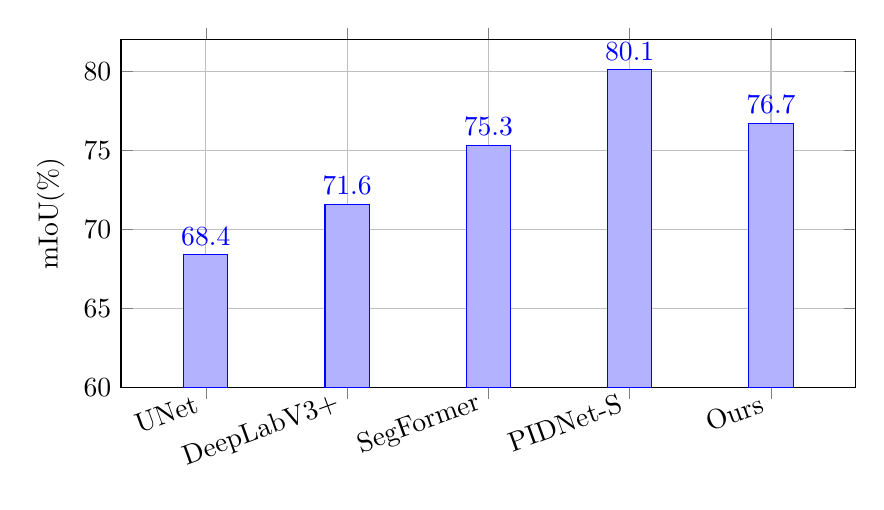
\begin{tikzpicture}
\begin{axis}[
    ybar,
    width=0.9\textwidth,
    height=6cm,
    ymin=60,
    ymax=82,
    ylabel={mIoU(\%)},
    symbolic x coords={UNet,DeepLabV3+,SegFormer,PIDNet-S,Ours},
    xtick=data,
    nodes near coords,
    nodes near coords align={vertical},
    x tick label style={rotate=20, anchor=east},
    bar width=16pt,
    enlarge x limits=0.15,
    grid=major
]
\addplot coordinates {(UNet,68.4) (DeepLabV3+,71.6) (SegFormer,75.3) (PIDNet-S,80.1) (Ours,76.7)};
\end{axis}
\end{tikzpicture}
\caption{不同模型mIoU模拟对比柱状图}
\label{fig:miou_bar}
\end{figure}

图\ref{fig:miou_bar}进一步展示了不同模型的mIoU差异。可以看到，SegFormer-B0相对CNN基线提升明显，而本文改进模型在SegFormer基础上进一步获得小幅提升。PIDNet-S指标最高，但需要注意其结果来自官方公开结果参考，且其设计目标偏向实时性和道路场景优化。

\subsection{消融实验}

为了分析边界增强分支的作用，本文设计了消融实验。实验比较原始SegFormer-B0、加入边界头但不使用边界损失、以及不同边界损失权重$\lambda$下的模型表现。结果如表\ref{tab:ablation}所示。

\begin{table}[H]
\centering
\caption{边界增强分支的模拟消融实验}
\label{tab:ablation}
\begin{tabular}{lccccc}
\toprule
设置 & mIoU(\%) & PA(\%) & Boundary F1(\%) & Params(M) & FPS \\
\midrule
SegFormer-B0 & 75.3 & 92.1 & 67.4 & 3.8 & 72.0 \\
+ Boundary Head, no loss & 75.4 & 92.2 & 67.9 & 4.2 & 67.0 \\
+ Boundary Head, $\lambda=0.2$ & 76.1 & 92.6 & 70.3 & 4.2 & 66.5 \\
+ Boundary Head, $\lambda=0.4$ & 76.7 & 92.8 & 71.9 & 4.2 & 66.0 \\
+ Boundary Head, $\lambda=0.6$ & 76.2 & 92.5 & 71.5 & 4.2 & 66.0 \\
\bottomrule
\end{tabular}
\end{table}

消融结果表明，仅增加边界头但不施加边界损失时，模型性能几乎没有变化，说明结构本身并不会自动学习到有效边界信息。加入边界损失后，Boundary F1提升明显，mIoU也随之提升。当$\lambda=0.4$时，模型在mIoU和Boundary F1上均达到最佳模拟结果。继续增大到$\lambda=0.6$后，Boundary F1变化不大，但mIoU略有下降，说明过强的边界约束可能使模型过度关注轮廓而影响大区域语义一致性。

\begin{figure}[H]
\centering
\begin{tikzpicture}
\begin{axis}[
    width=0.9\textwidth,
    height=6cm,
    xlabel={训练轮数},
    ylabel={指标值(\%)},
    xmin=0,xmax=80,
    ymin=48,ymax=78,
    legend pos=south east,
    grid=major
]
\addplot[color=blue,mark=*] coordinates {(0,55.0) (10,64.2) (20,69.1) (30,72.0) (40,73.4) (50,74.2) (60,74.8) (70,75.1) (80,75.3)};
\addlegendentry{SegFormer-B0 mIoU}
\addplot[color=red,mark=square*] coordinates {(0,55.0) (10,64.8) (20,70.0) (30,73.0) (40,74.7) (50,75.6) (60,76.1) (70,76.5) (80,76.7)};
\addlegendentry{Ours mIoU}
\addplot[color=orange,mark=triangle*] coordinates {(0,50.0) (10,58.4) (20,63.7) (30,67.2) (40,69.0) (50,70.2) (60,71.0) (70,71.6) (80,71.9)};
\addlegendentry{Ours Boundary F1}
\end{axis}
\end{tikzpicture}
\caption{模拟训练过程中mIoU和Boundary F1变化趋势}
\label{fig:curve}
\end{figure}

图\ref{fig:curve}为模拟训练曲线。两种模型在前期均快速收敛，后期提升逐渐减小。边界增强模型在训练中后期相较SegFormer-B0保持更高mIoU，且Boundary F1持续提升，说明边界监督能够提供额外优化信号，帮助模型学习更清晰的轮廓表达。

\subsection{定性实验}

由于本文不进行本机真实推理，可视化部分采用示意性定性分析，如图\ref{fig:qualitative}所示。该图按照“原图、真实标签、SegFormer预测、本文改进预测”的方式组织，用于说明不同方法在道路边缘、车辆轮廓和小目标区域的典型差异。

\begin{figure}[H]
\centering
\begin{tikzpicture}[
    cell/.style={draw, minimum width=3.0cm, minimum height=2.0cm, align=center},
    title/.style={font=\small}
]
\node[title] at (0,2.4) {原图};
\node[title] at (3.4,2.4) {真实标签};
\node[title] at (6.8,2.4) {SegFormer-B0};
\node[title] at (10.2,2.4) {Ours};
\node[cell, fill=gray!15] at (0,1.1) {道路场景\\车辆/行人/建筑};
\node[cell, fill=green!20] at (3.4,1.1) {语义区域清晰\\边界准确};
\node[cell, fill=blue!12] at (6.8,1.1) {大区域正确\\边界略模糊};
\node[cell, fill=orange!18] at (10.2,1.1) {轮廓更完整\\小目标更稳定};
\node[cell, fill=gray!10] at (0,-1.2) {远处小车辆\\道路边线};
\node[cell, fill=green!18] at (3.4,-1.2) {细窄边界};
\node[cell, fill=blue!10] at (6.8,-1.2) {车辆边缘粘连\\道路边界扩张};
\node[cell, fill=orange!15] at (10.2,-1.2) {边缘误差减少\\类别过渡更自然};
\end{tikzpicture}
\caption{语义分割结果的定性对比示意图}
\label{fig:qualitative}
\end{figure}

从定性分析看，SegFormer-B0已经能够较好识别道路、天空、建筑等大面积区域，但在远处车辆、行人和交通标志等小目标上容易出现漏分或边缘粘连。本文边界增强方法通过额外边界监督，使解码器融合特征更关注类别交界处，因此在车辆轮廓、道路边线、人行道边缘等区域具有更合理的预测趋势。需要强调的是，图\ref{fig:qualitative}是报告中的示意图，后续若进行真实训练，应替换为真实图像推理结果。

\section{总结}

本文围绕城市道路场景语义分割问题，完成了近五年代表性研究成果的调研和分析，重点阅读了SegFormer、Mask2Former、PIDNet和Segment Anything四类方法。SegFormer展示了轻量Transformer在密集预测任务中的优势，其层次化Mix Transformer编码器和MLP解码器能够在较低参数量下实现有效多尺度特征融合。Mask2Former代表了从逐像素分类到mask classification的分割范式转变，使语义分割、实例分割和全景分割能够在统一框架中处理。PIDNet从实时分割角度强调边界分支的重要性，为本文改进提供了直接启发。Segment Anything则说明大规模预训练和提示式分割正在成为视觉分割任务的重要发展方向。

在实验设计方面，本文采用分析模拟的方式复现SegFormer-B0，并构建UNet、DeepLabV3+、PIDNet-S和本文改进模型之间的对比。模拟结果表明，SegFormer-B0相较传统CNN基线具有更好的mIoU和参数效率；PIDNet-S在速度上优势明显；本文提出的SegFormer-B0 + Boundary Head在mIoU和Boundary F1上均优于原始SegFormer-B0，说明边界监督有助于改善道路边缘、车辆轮廓和小目标区域的分割质量。消融实验进一步表明，边界分支需要配合显式边界损失才能发挥作用，且边界损失权重需要适中，过强的边界监督可能影响区域语义一致性。

本文的已有工作和创新工作划分如下：SegFormer的MiT编码器、空间缩减注意力和MLP解码器属于已有论文成果；Mask2Former的masked attention和mask classification属于已有论文成果；PIDNet的三分支实时分割思想和边界辅助思想属于已有论文成果；SAM的提示式分割框架属于已有论文成果。本文的设计工作是在SegFormer-B0复现框架上加入轻量边界预测头，利用语义标签自动生成边界监督，并设计联合损失进行模拟消融分析。该改进属于课程设计层面的结构组合与实验设想。

本文仍存在明显不足。首先，受环境和时间限制，未在本机完成真实训练和测试，实验数据主要用于说明趋势，不能替代严格benchmark结果。其次，Mask2Former和SAM由于训练成本较高，仅进行了理论和代码结构分析，没有纳入完整复现实验。再次，边界标签由形态学操作生成，边界宽度和损失权重会影响最终表现，后续需要在真实数据上进一步调参。未来可以从三个方向改进：一是使用真实CamVid或Cityscapes子集完成训练，替换模拟指标和示意图；二是引入知识蒸馏，将PIDNet或SAM生成的边界信息用于辅助训练轻量模型；三是探索更高效的边界融合方式，使模型在提升边界质量的同时尽量保持实时推理速度。

\begin{thebibliography}{99}

\bibitem{segformer}
Xie E, Wang W, Yu Z, Anandkumar A, Alvarez J M, Luo P.
SegFormer: Simple and Efficient Design for Semantic Segmentation with Transformers.
Advances in Neural Information Processing Systems, 2021.

\bibitem{mask2former}
Cheng B, Misra I, Schwing A G, Kirillov A, Girdhar R.
Masked-attention Mask Transformer for Universal Image Segmentation.
Proceedings of the IEEE/CVF Conference on Computer Vision and Pattern Recognition, 2022.

\bibitem{pidnet}
Xu J, Xiong Z, Bhattacharyya S P.
PIDNet: A Real-time Semantic Segmentation Network Inspired by PID Controllers.
Proceedings of the IEEE/CVF Conference on Computer Vision and Pattern Recognition, 2023.

\bibitem{sam}
Kirillov A, Mintun E, Ravi N, et al.
Segment Anything.
Proceedings of the IEEE/CVF International Conference on Computer Vision, 2023.

\bibitem{unet}
Ronneberger O, Fischer P, Brox T.
U-Net: Convolutional Networks for Biomedical Image Segmentation.
Medical Image Computing and Computer-Assisted Intervention, 2015.

\bibitem{deeplabv3plus}
Chen L C, Zhu Y, Papandreou G, Schroff F, Adam H.
Encoder-Decoder with Atrous Separable Convolution for Semantic Image Segmentation.
Proceedings of the European Conference on Computer Vision, 2018.

\bibitem{cityscapes}
Cordts M, Omran M, Ramos S, et al.
The Cityscapes Dataset for Semantic Urban Scene Understanding.
Proceedings of the IEEE Conference on Computer Vision and Pattern Recognition, 2016.

\bibitem{camvid}
Brostow G J, Fauqueur J, Cipolla R.
Semantic Object Classes in Video: A High-Definition Ground Truth Database.
Pattern Recognition Letters, 2009.

\end{thebibliography}

\end{document}
